% =============================================================================
% Punto 4 — Análisis de frecuencias mediante Fourier (Rol C)
% Cuenca Río Maipo en El Manzano (CAMELS-CL 5710001)
% Figuras y tablas: scripts/13_p4_1_preparacion_espectral.py y
%                   scripts/14_p4_2_espectros_interpretacion.py
% Compilar desde documentos/:  pdflatex punto4_fourier_analisis.tex
% LAS REFERENCIAS HAN SIDO CONTRASTADAS CON LA FUENTE ORIGINAL.
% =============================================================================
\documentclass[11pt,letterpaper]{article}
\usepackage[utf8]{inputenc}
\usepackage[T1]{fontenc}
\usepackage[spanish,es-nodecimaldot,es-noshorthands]{babel}
\usepackage{lmodern}
\usepackage[margin=2.3cm]{geometry}
\usepackage{amsmath,amssymb}
\usepackage{graphicx}
\usepackage{booktabs}
\usepackage{float}
\usepackage{caption}
\usepackage[numbers,sort&compress]{natbib}
\usepackage[hidelinks]{hyperref}
\graphicspath{{../figuras/}}
\captionsetup{font=small,labelfont=bf}

\title{Punto 4. Análisis de frecuencias mediante Fourier\\
\large Río Maipo en El Manzano (CAMELS-CL 5710001) --- Rol C}
\author{Tarea 1 de Hidrología, UNAL Medellín}
\date{}

\begin{document}
\sloppy
\maketitle

\section{Preparación de las series y cálculo (4.1)}

Se usa la secuencia mensual cronológica, con $\Delta t=1$ mes, y no las doce medias climatológicas. Para que el
ciclo anual quepa un número entero de veces y se reduzca la fuga del pico anual, se eligieron tramos de años
hidrológicos completos (abril--marzo):

\begin{itemize}
\item \textbf{Registro completo} (1980-04 a 2020-03, $N=480$, 40 ciclos anuales) para $P_L$ y $\overline{Q}$.
\item \textbf{Periodo común} (2001-04 a 2020-03, $N=228$, 19 ciclos anuales) para $P_L$, $P_I$, $\overline{Q}$ y $T$,
que permite comparar fuentes sobre los mismos meses.
\end{itemize}

Así, $\Delta f=1/N$ es $2.08\times10^{-3}$ y $4.39\times10^{-3}$ ciclos/mes; la frecuencia de Nyquist es 0.5
ciclos/mes (periodo mínimo de 2 meses) y el periodo más largo representable es $N$ meses, aunque con un solo
ciclo observado. La frecuencia cero (la media) se excluye.

\paragraph{Vacíos.} Solo el caudal tiene faltantes: 14 meses en el tramo completo y 8 en el común
(2015-04 a 2015-11). No se eliminaron (eso concatenaría meses no consecutivos) ni se rellenaron con ceros. Se
interpoló linealmente la \emph{anomalía} entre los meses válidos vecinos y se le sumó la climatología del mes,
y cada valor rellenado quedó marcado (Figura~\ref{fig:prep}). El efecto se evaluó con el tramo continuo
1990-12 a 2014-11 ($N=288$) y con un periodograma de Lomb--Scargle \citep{Lomb1976,Scargle1982} sobre los
datos sin rellenar.

\paragraph{Transformaciones.} C: serie original centrada (conserva el ciclo anual); A: anomalía respecto de la
climatología mensual fija 2000-06/2020-03, centrada en el tramo (la referencia no coincide con el tramo
completo y su media residual contaminaría las bajas frecuencias); AD: A sin la tendencia lineal OLS del tramo,
para evaluar la sensibilidad a la tendencia identificada en el punto 3 ($-10.5$~mm/mes por década en $P_L$ y
$-18.0$~m$^3$/s por década en $\overline{Q}$ en el tramo completo).

\paragraph{Estimadores y convención.} Se calcula la densidad espectral de potencia unilateral
\begin{equation}
P(f_k)=\frac{2\,\Delta t}{\sum_n w_n^2}\left|\sum_{n=0}^{N-1} w_n\,x_n\,e^{-i2\pi kn/N}\right|^2,\qquad
f_k=\frac{k}{N\Delta t},\quad 0<f_k<0.5,
\end{equation}
en unidades de (unidad de la variable)$^2$/(ciclo/mes), de modo que $\sum_k P(f_k)\,\Delta f$ es igual a la
varianza (Parseval, verificado con cociente 1.00). Se comparan tres estimadores: periodograma sin ventana
(boxcar, máxima resolución y mayor fuga), periodograma con ventana Hann (estimador principal, que reduce la
fuga a costa de ensanchar el lóbulo principal a $\sim2\Delta f$) y Welch con segmentos Hann de 120 meses y 50\,\%
de solapamiento \citep{Welch1967,Harris1978}, que reduce la varianza del estimador pero no resuelve periodos
mayores de unos 10 años. No se usó relleno con ceros.

\begin{figure}[H]
\centering
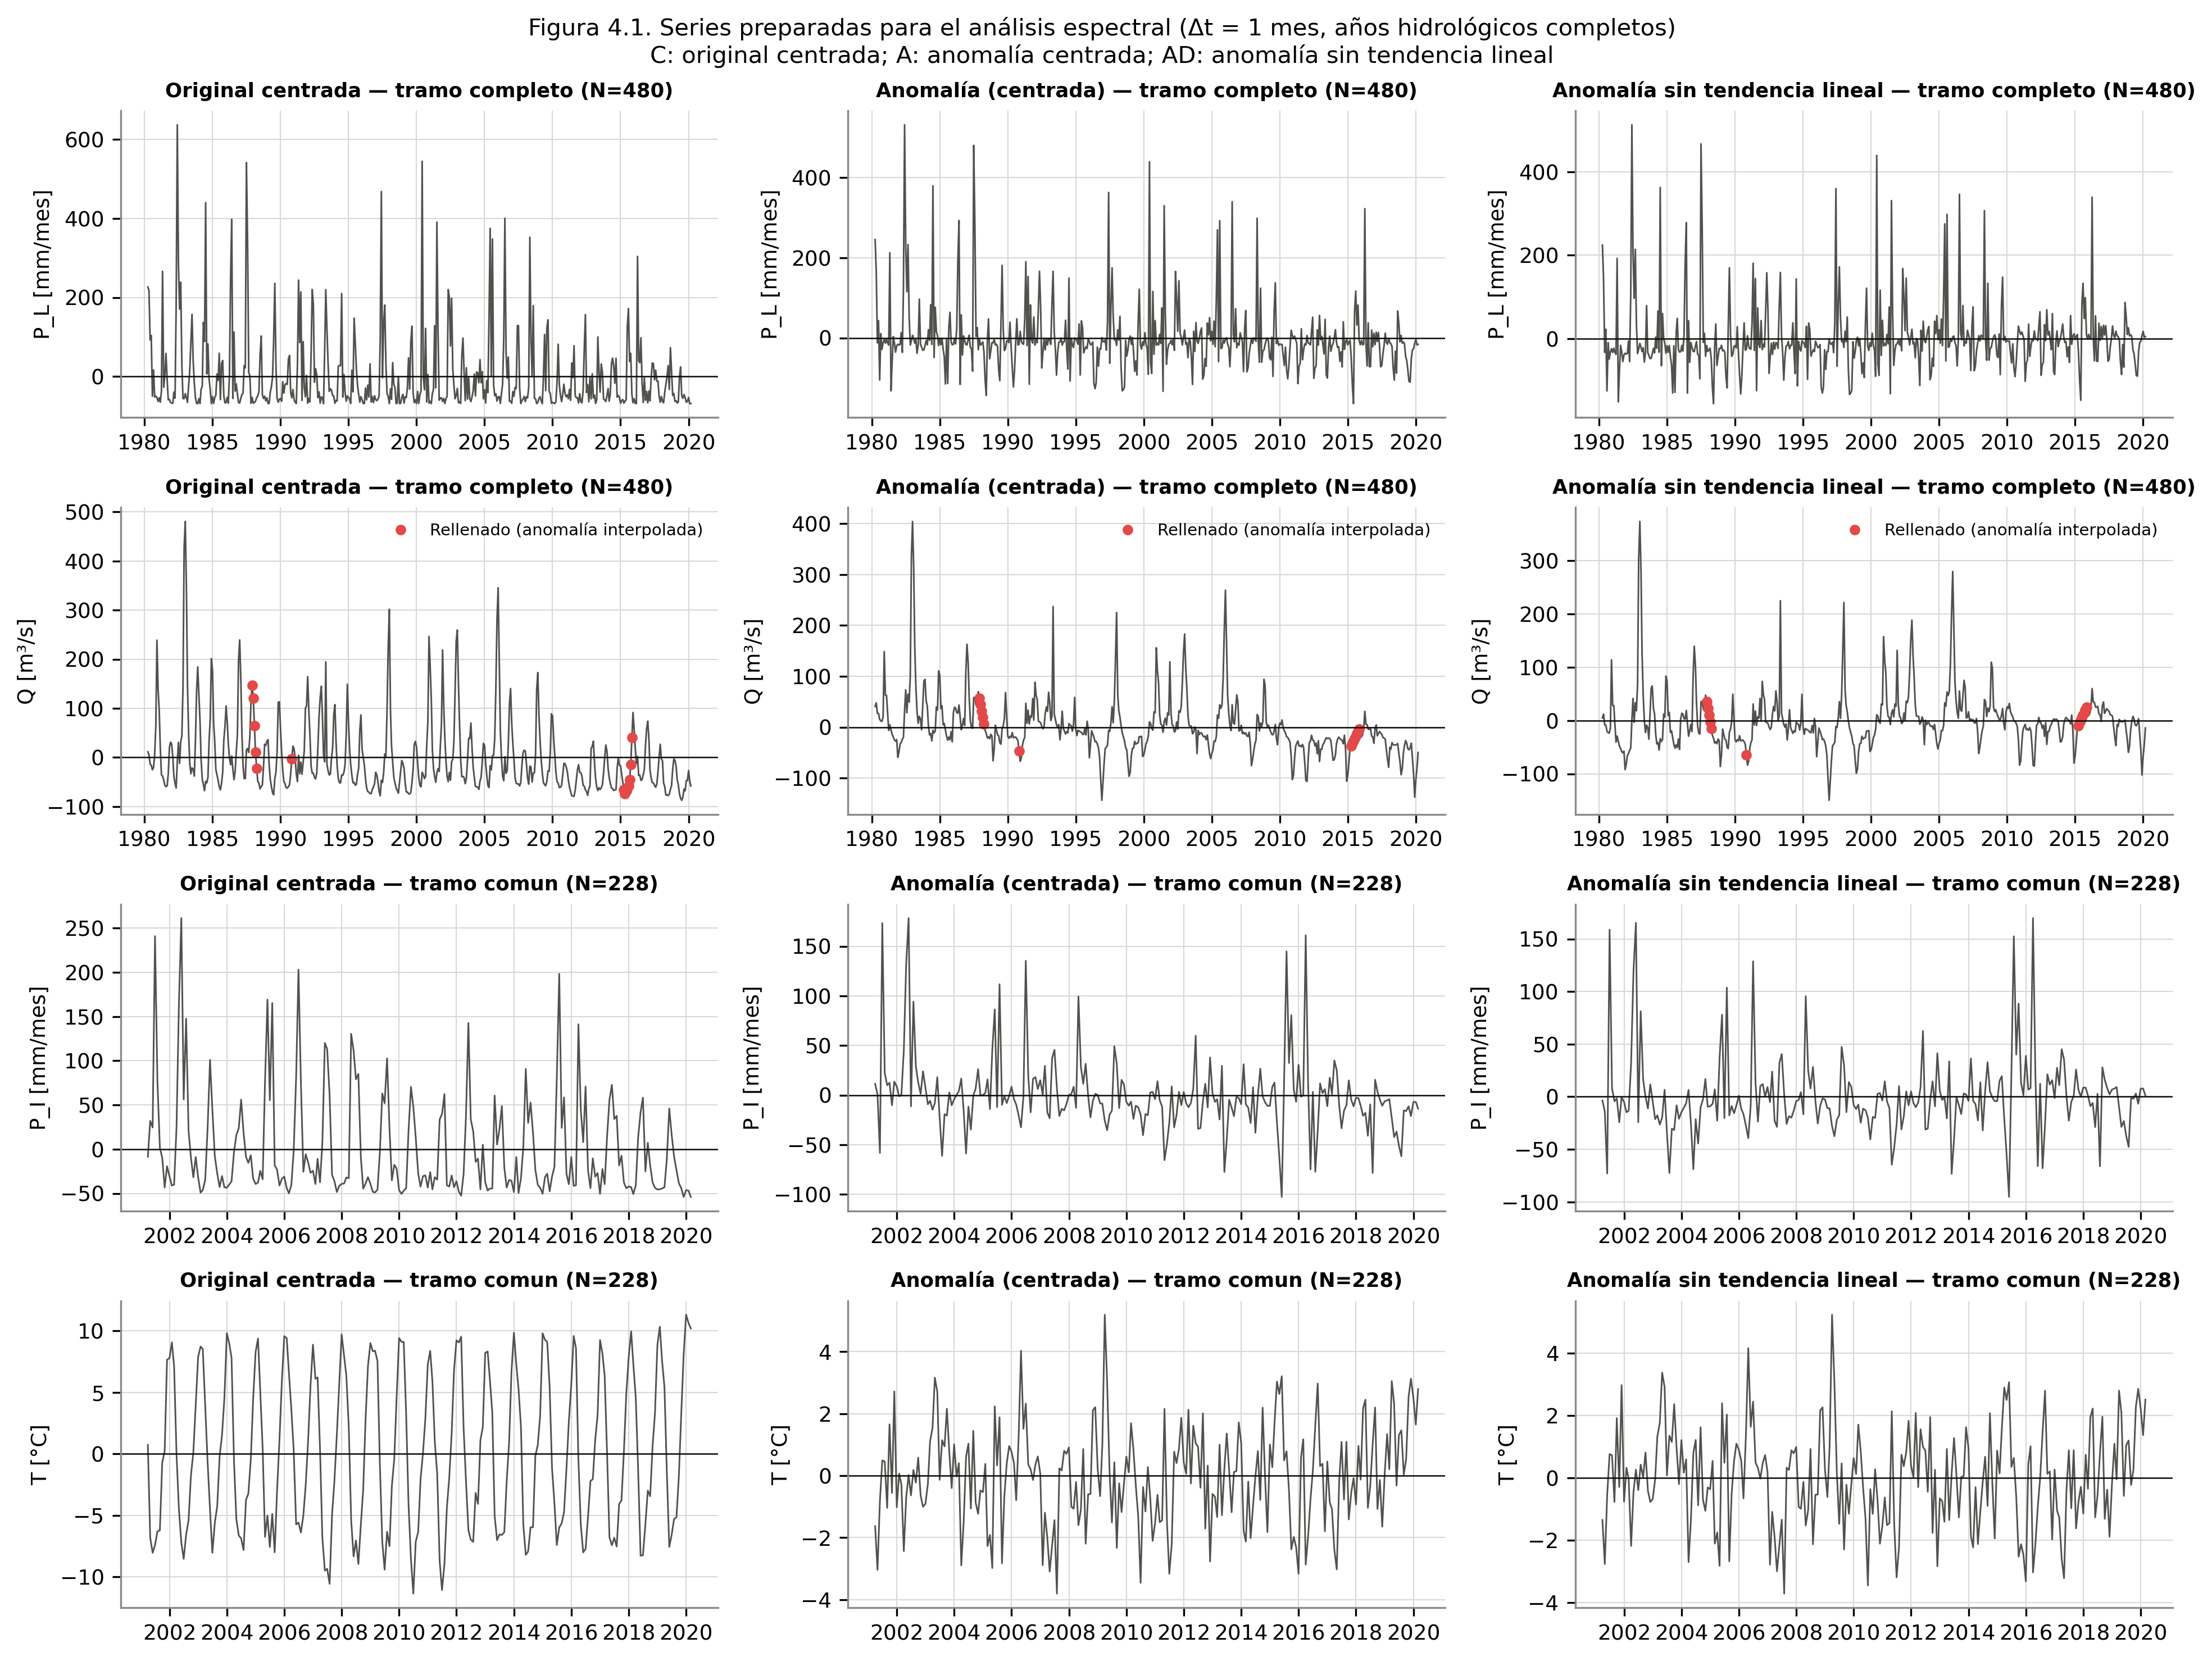
\includegraphics[width=\textwidth]{figura_4_1_series_preparadas.png}
\caption{Series preparadas para el análisis espectral: original centrada (C), anomalía (A) y anomalía sin
tendencia (AD). Puntos rojos: meses de caudal rellenados por interpolación de la anomalía. Script
\texttt{13\_p4\_1\_preparacion\_espectral.py}.}
\label{fig:prep}
\end{figure}

\paragraph{Significancia.} Un máximo del periodograma no demuestra por sí solo una periodicidad. Para las
anomalías se adoptó como hipótesis nula un ruido rojo AR(1) con el coeficiente de autocorrelación de rezago 1
y la varianza de cada serie \citep{Gilman1963,Torrence1998}. Se simularon 1000 series AR(1) de igual longitud y
se procesaron con el mismo estimador para obtener dos umbrales del 95\,\%: uno \emph{puntual} (por frecuencia) y
otro \emph{global}, que usa el percentil 95 del máximo cociente entre el periodograma y el fondo sobre todas las
frecuencias y corrige así la búsqueda entre unas 100--240 frecuencias. A las series originales no se les aplica
esta prueba: su ciclo anual es determinista y no se puede tratar como ruido rojo.

\section{Espectros e interpretación (4.2)}

\begin{figure}[H]
\centering
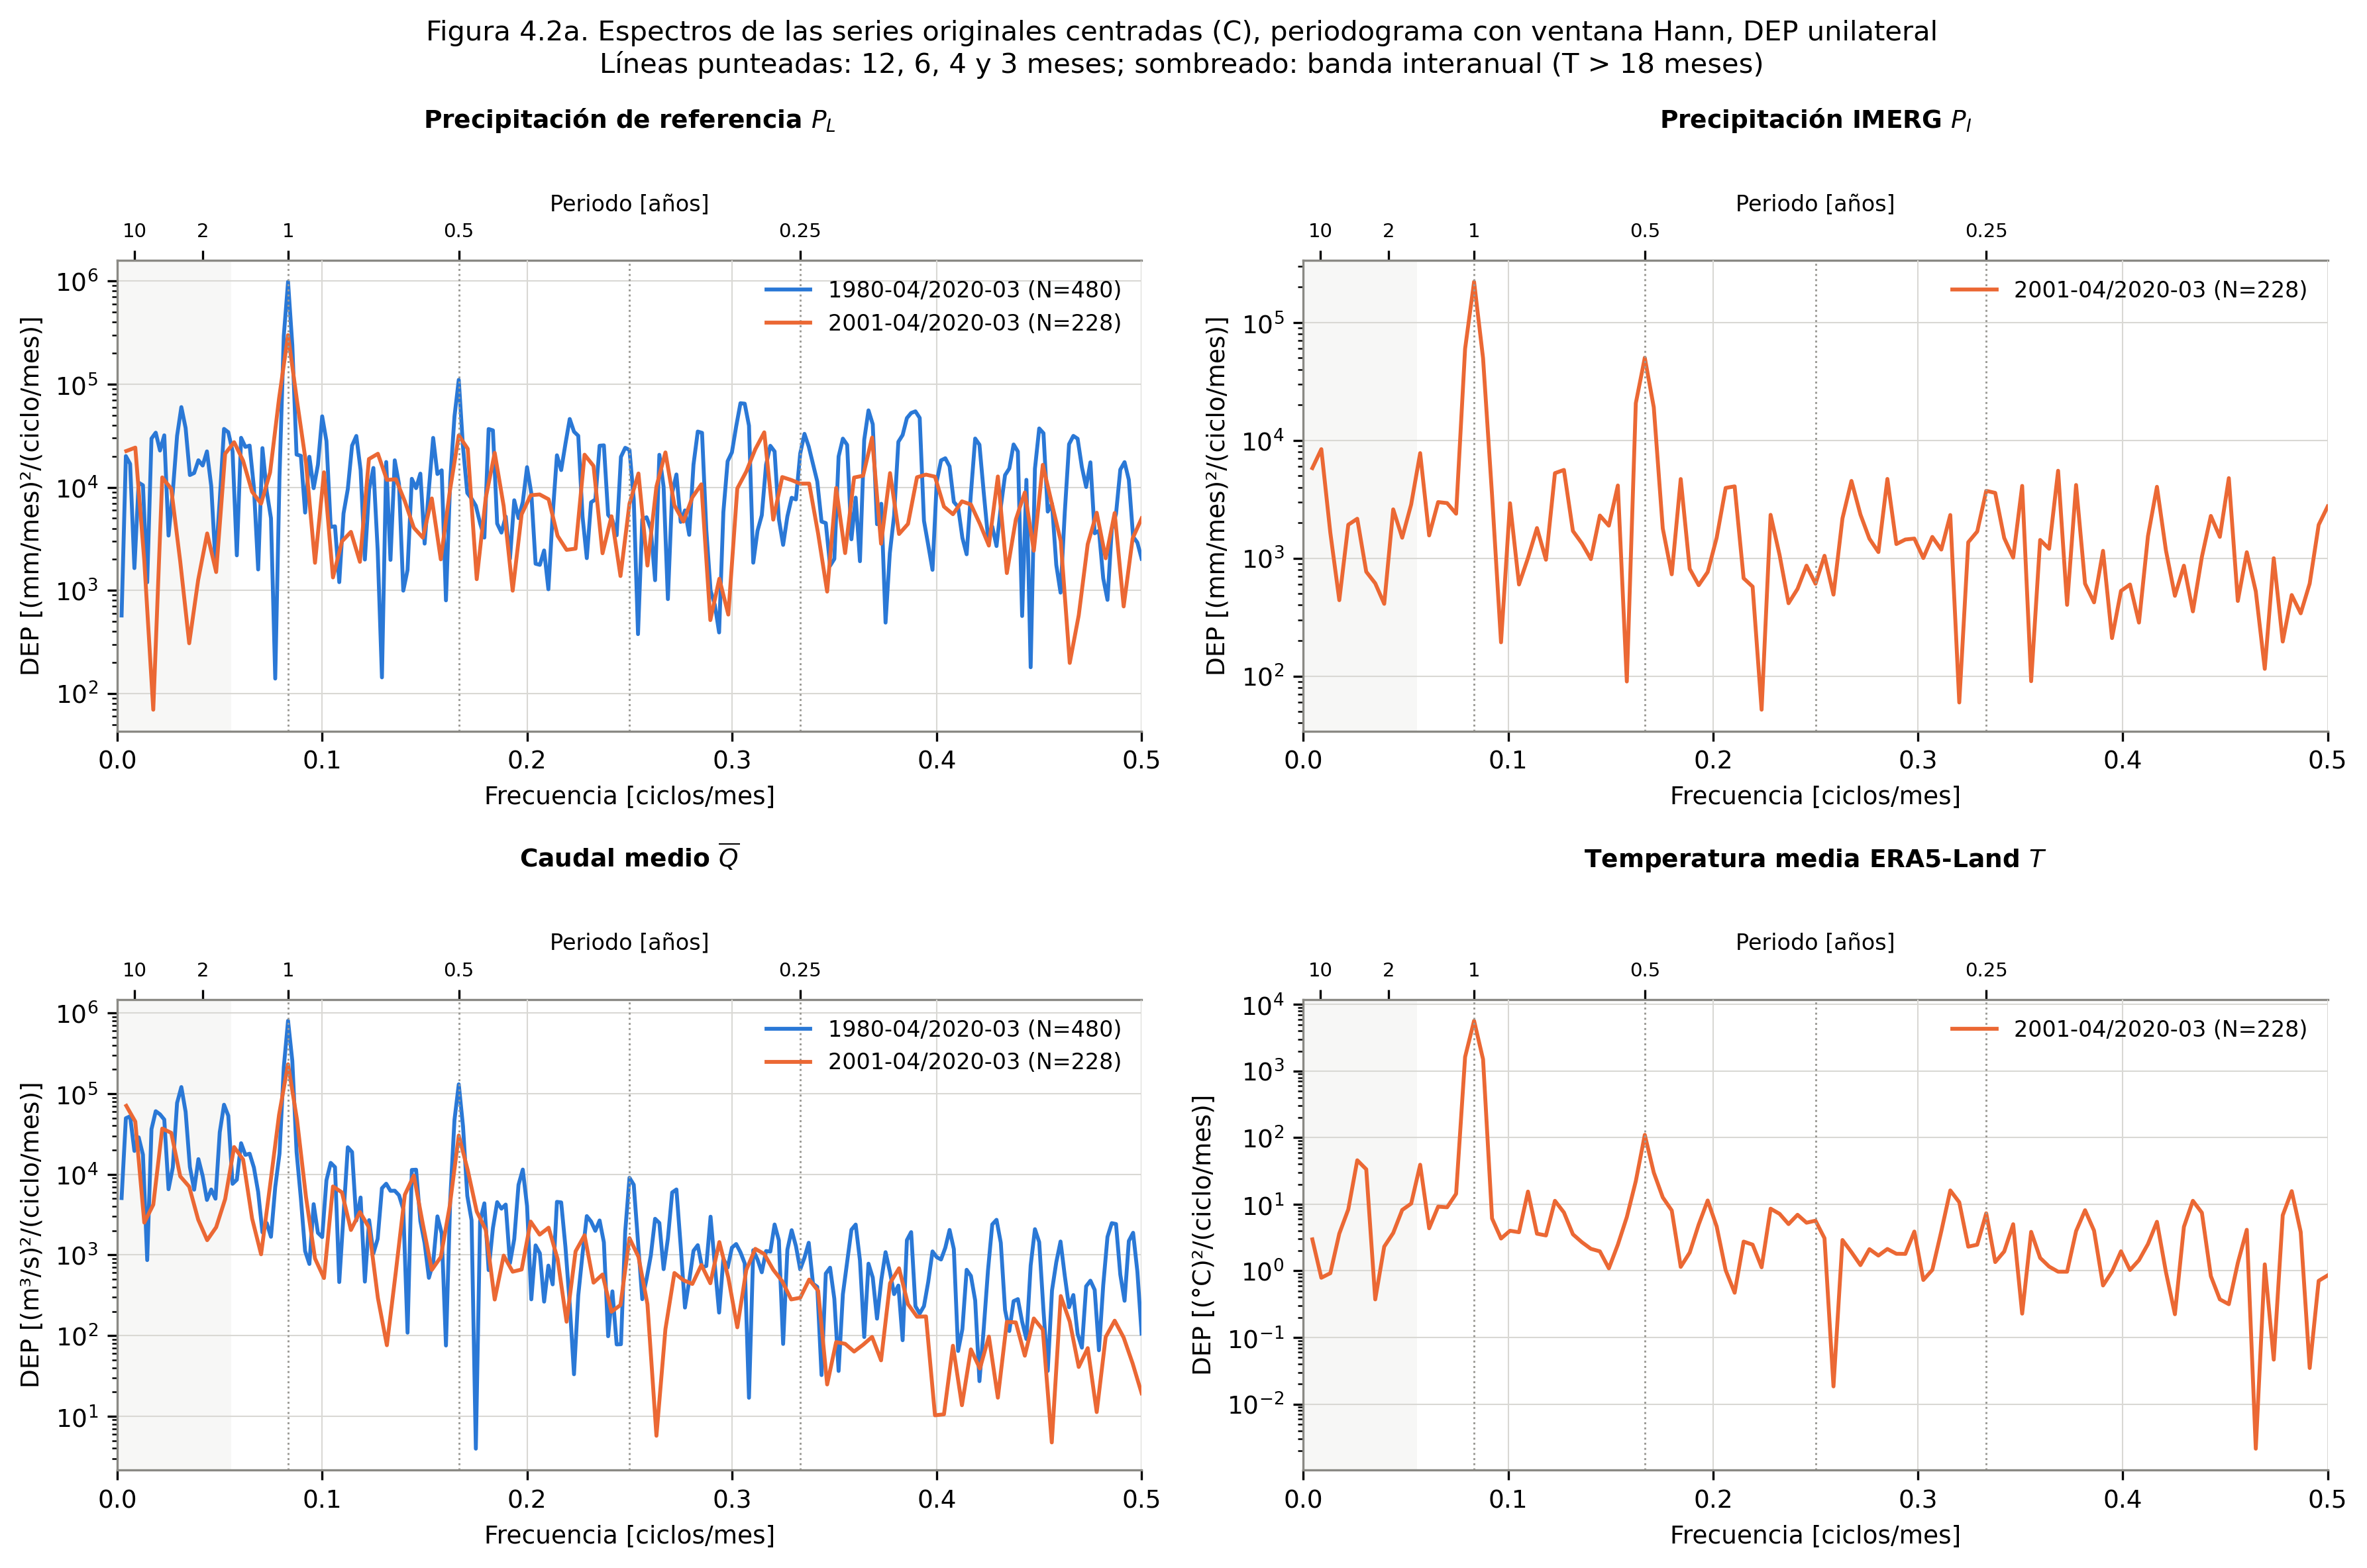
\includegraphics[width=\textwidth]{figura_4_2a_espectros_originales.png}
\caption{Espectros de las series originales centradas (C), periodograma Hann, densidad espectral unilateral.
Eje superior: periodo en años. Líneas punteadas: 12, 6, 4 y 3 meses; sombreado: banda interanual
($T>18$ meses). Script \texttt{14\_p4\_2\_espectros\_interpretacion.py}.}
\label{fig:orig}
\end{figure}

\begin{figure}[H]
\centering
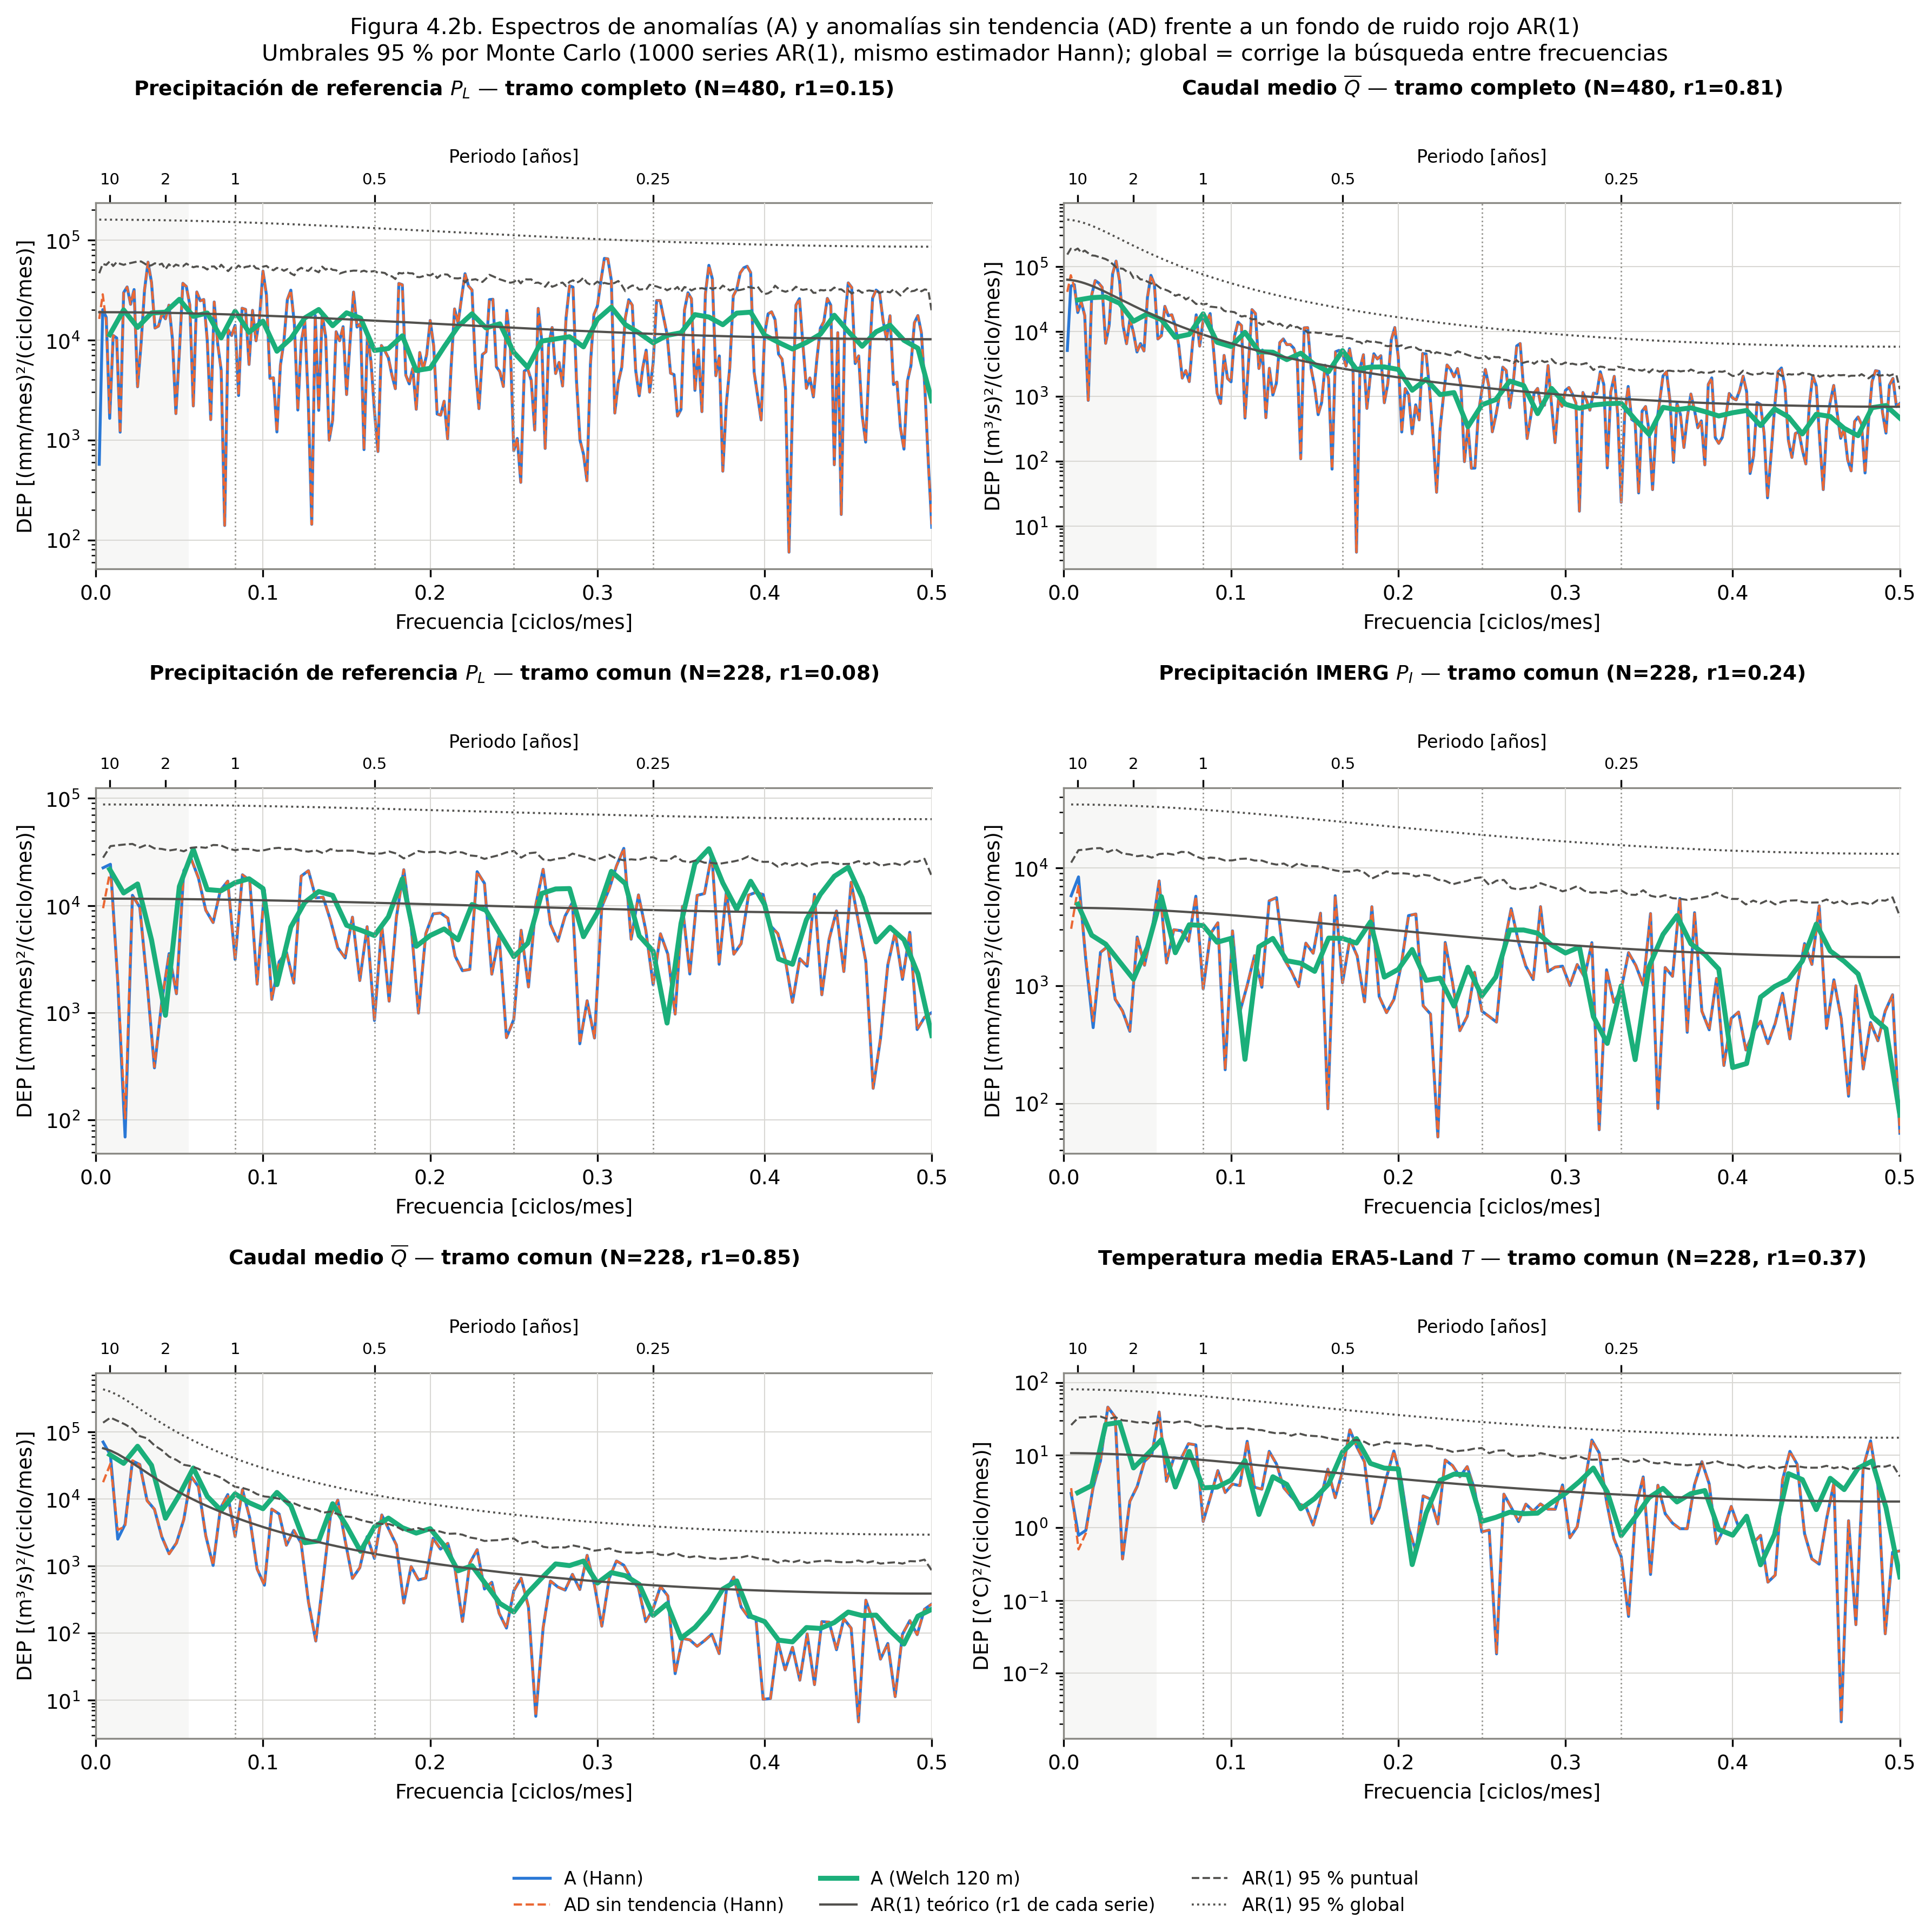
\includegraphics[width=\textwidth]{figura_4_2b_espectros_anomalias_ar1.png}
\caption{Espectros de anomalías (A, azul), anomalías sin tendencia (AD, naranja) y Welch (verde) frente al fondo
AR(1) (gris) y sus umbrales del 95\,\% puntual (discontinuo) y global (punteado), obtenidos por Monte Carlo.}
\label{fig:anom}
\end{figure}

\subsection{Picos y bandas dominantes}

La Tabla~\ref{tab:picos} resume los picos principales (tabla completa en
\texttt{figuras/tabla\_4\_2\_picos\_espectrales.csv}) y la Tabla~\ref{tab:bandas}, la fracción de la varianza
en cada banda. Como la resolución es $\Delta f=1/N$, cada periodo es en realidad un intervalo: por ejemplo, el
pico de 32 meses del tramo completo representa periodos entre 30 y 34 meses y solo 15 ciclos observados, y el
de 38 meses de $T$ abarca de 33 a 46 meses con apenas 6 ciclos. No se les asigna mayor precisión.

\begin{table}[H]
\centering\small
\caption{Picos espectrales principales (periodograma Hann). El intervalo de periodo corresponde a
$f\pm\Delta f$; ``Ciclos'' $=Nf$. AR(1) indica si el pico supera el umbral del 95\,\% puntual (P) o global (G).}
\label{tab:picos}
\begin{tabular}{llllrrl}
\toprule
Variable & Tramo & Transf. & Periodo [meses] & Intervalo & Ciclos & AR(1) \\
\midrule
$P_L$ & completo & C & 12.0 & 11.7--12.3 & 40 & -- \\
$P_L$ & completo & C & 6.0 & 5.9--6.1 & 80 & -- \\
$P_L$ & completo & A & 32.0 & 30.0--34.3 & 15 & P, no G \\
$P_L$ & completo & A & 3.3; 2.7; 2.6 & -- & 146--187 & P, no G \\
$\overline{Q}$ & completo & C & 12.0 & 11.7--12.3 & 40 & -- \\
$\overline{Q}$ & completo & C & 53.3 & 48.0--60.0 & 9 & -- \\
$\overline{Q}$ & completo & A & 32.0 & 30.0--34.3 & 15 & P, no G \\
$\overline{Q}$ & completo & A & 19.2 & 18.5--20.0 & 25 & P, no G \\
$P_I$ & común & C & 12.0 & 11.4--12.7 & 19 & -- \\
$P_I$ & común & C & 6.0 & 5.8--6.2 & 38 & -- \\
$\overline{Q}$ & común & A & 6.9 & 6.7--7.1 & 33 & P, no G \\
$T$ & común & C & 12.0 & 11.4--12.7 & 19 & -- \\
$T$ & común & A & 38.0; 17.5 & 32.6--45.6; 16.3--19.0 & 6; 13 & P, no G \\
\bottomrule
\end{tabular}
\end{table}

\begin{table}[H]
\centering\small
\caption{Fracción de la varianza por banda (periodograma Hann). Interanual: $T>18$ meses; anual: 10.5--14
meses; semianual: 5.25--7 meses; resto: frecuencias intraanuales no armónicas.
Fuente: \texttt{figuras/tabla\_4\_2\_fracciones\_banda.csv}.}
\label{tab:bandas}
\begin{tabular}{lllrrrr}
\toprule
Variable & Tramo & Transf. & Interanual & Anual & Semianual & Resto \\
\midrule
$P_L$ & completo & C & 0.10 & 0.32 & 0.08 & 0.50 \\
$P_L$ & completo & A & 0.15 & 0.04 & 0.07 & 0.74 \\
$\overline{Q}$ & completo & C & 0.30 & 0.46 & 0.10 & 0.14 \\
$\overline{Q}$ & completo & A & 0.60 & 0.06 & 0.06 & 0.28 \\
$P_L$ & común & C & 0.07 & 0.34 & 0.09 & 0.51 \\
$P_I$ & común & C & 0.05 & 0.55 & 0.17 & 0.24 \\
$\overline{Q}$ & común & C & 0.30 & 0.47 & 0.09 & 0.14 \\
$T$ & común & C & 0.01 & 0.93 & 0.02 & 0.04 \\
$P_L$ & común & A & 0.11 & 0.08 & 0.08 & 0.73 \\
$P_I$ & común & A & 0.15 & 0.08 & 0.13 & 0.65 \\
$\overline{Q}$ & común & A & 0.56 & 0.10 & 0.08 & 0.25 \\
$T$ & común & A & 0.21 & 0.07 & 0.12 & 0.60 \\
\bottomrule
\end{tabular}
\end{table}

\subsection{Bandas anual, semianual e interanual}

\paragraph{Series originales.} En las cuatro variables domina la banda anual (Figura~\ref{fig:orig}), que es el
único pico inequívoco del análisis: 40 ciclos en el registro completo y una altura de varios órdenes de
magnitud sobre el fondo. Su peso varía mucho: 93\,\% de la varianza en $T$, cuyo ciclo es casi sinusoidal y lo
controla la radiación; 46--47\,\% en $\overline{Q}$, 55\,\% en $P_I$ y solo 32--34\,\% en $P_L$. La precipitación de
referencia concentra la mitad de su varianza en frecuencias intraanuales no armónicas, porque llega en pocos
eventos frontales invernales muy irregulares (asimetría +2.8 según el rol A). El pico de 6 meses de la
precipitación y del caudal no indica un segundo proceso: es el armónico de un ciclo anual no sinusoidal (un
invierno lluvioso de unos cinco meses y un verano casi seco, o un hidrograma de deshielo asimétrico). Este
armónico es mayor en $P_I$ (17\,\%) que en $P_L$ (8--9\,\%); en el periodo común, IMERG reproduce un ciclo
estacional más regular y menos variabilidad entre eventos que la referencia, lo que concuerda con su
subestimación de los extremos invernales documentada en el punto 2.

\paragraph{Al retirar la climatología.} Las bandas anual y semianual se reducen a un 4--10\,\% de la varianza
de las anomalías (Tabla~\ref{tab:bandas}); lo que queda refleja que la amplitud del ciclo cambia de un año a
otro, no un ciclo determinista. La varianza se redistribuye de forma muy distinta según la variable:
\begin{itemize}
\item En $P_L$ y $P_I$ el espectro de anomalías es casi plano (ruido casi blanco: $r_1=0.15$ y $0.24$; pendiente
log--log de $+0.18$ y $-0.08$ en $f<1/12$). La banda interanual solo reúne el 11--15\,\% de la varianza.
\item En $\overline{Q}$ el espectro es rojo: $r_1=0.81$ (0.85 en el periodo común), pendiente log--log de $-0.33$ a
$-0.79$ y 56--60\,\% de la varianza de las anomalías en periodos de más de 18 meses, con una caída marcada de
la potencia a altas frecuencias (Figura~\ref{fig:norm}).
\item En $T$ las anomalías tienen persistencia moderada ($r_1=0.37$) y un 21\,\% de varianza interanual.
\end{itemize}

\begin{figure}[H]
\centering
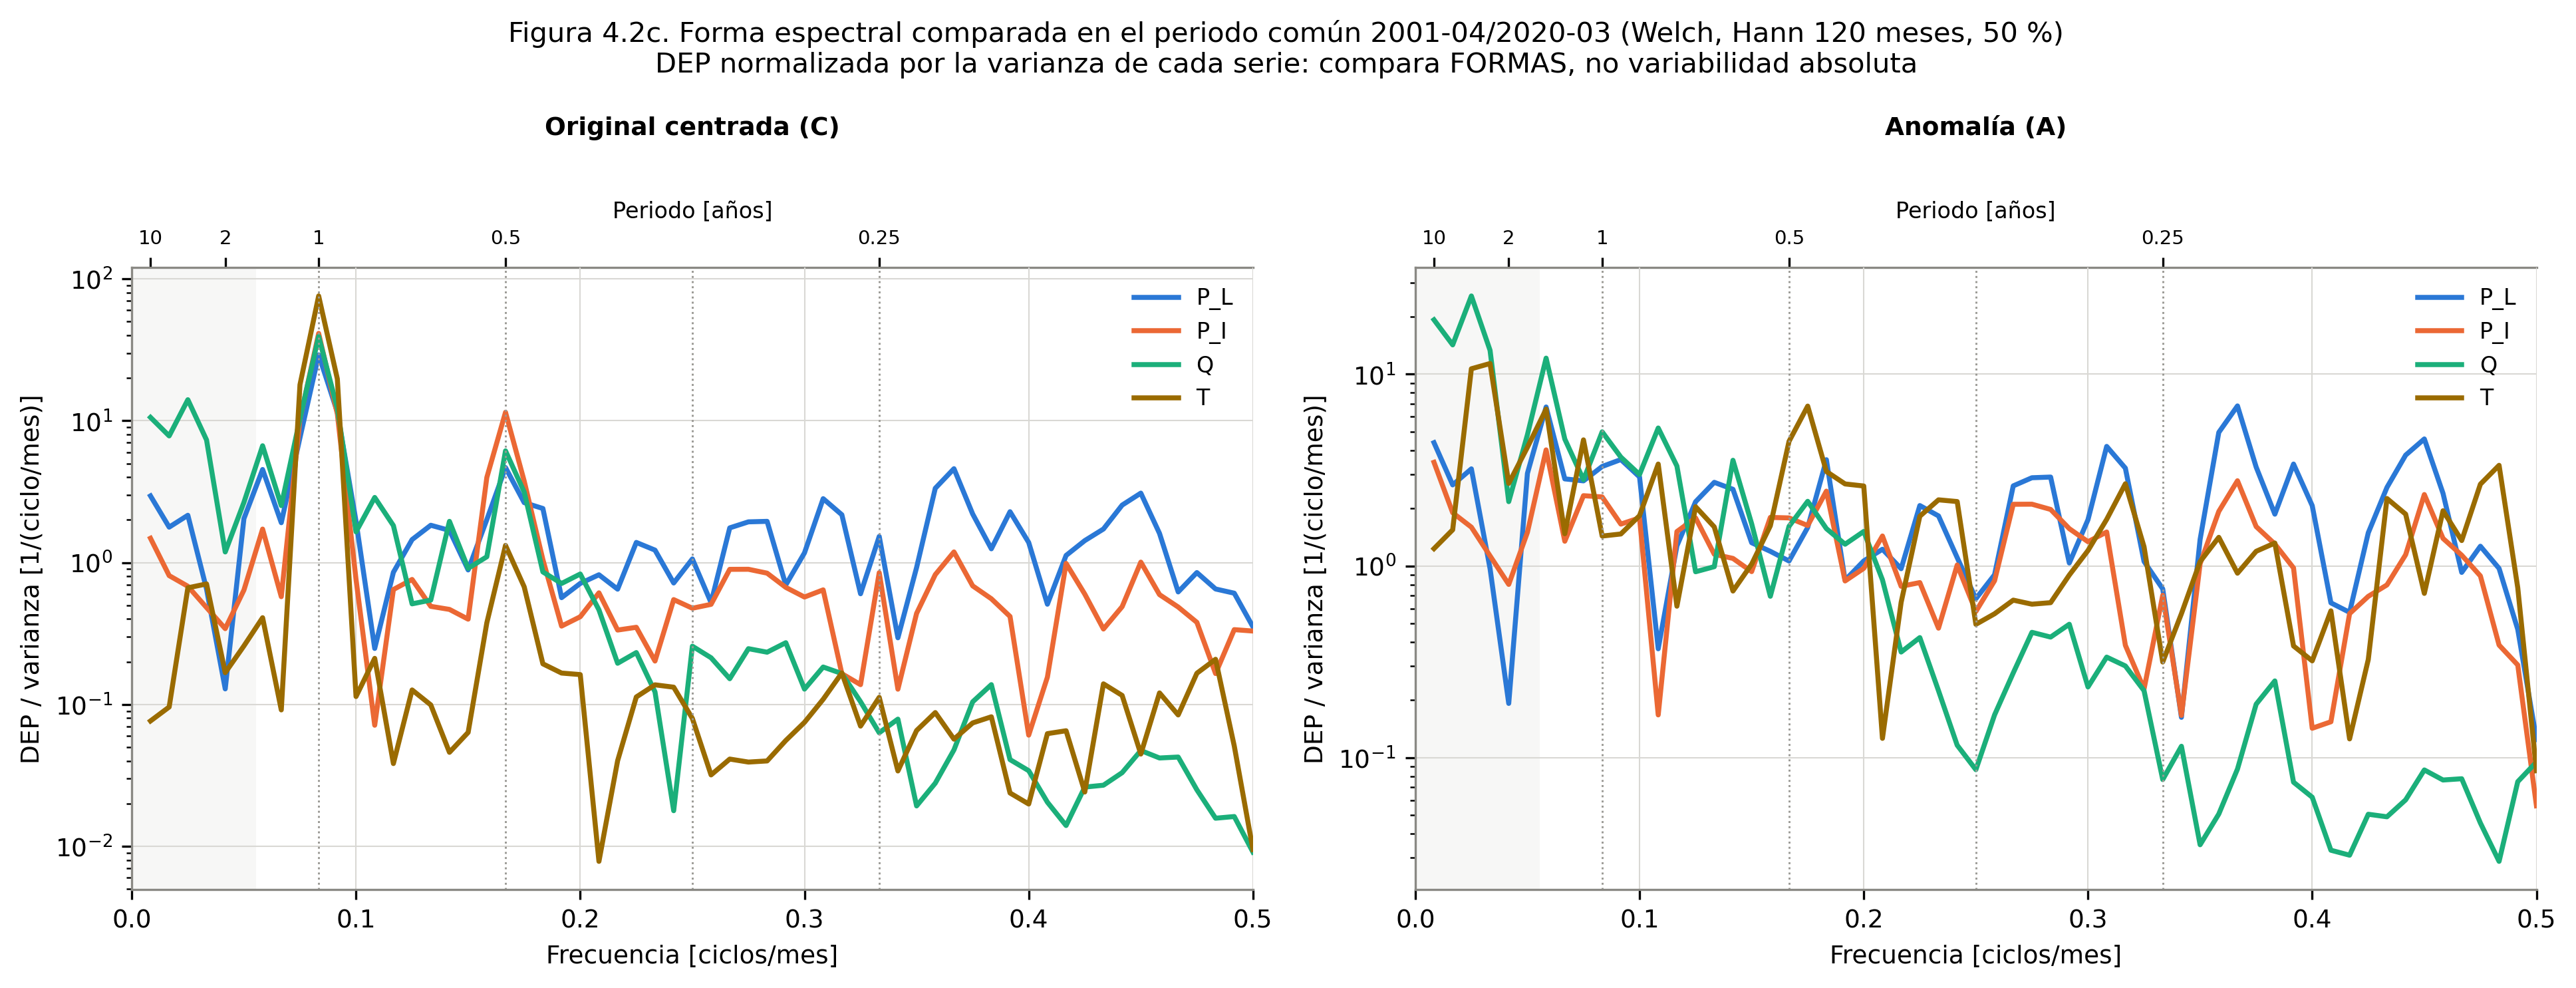
\includegraphics[width=\textwidth]{figura_4_2c_espectros_normalizados.png}
\caption{Forma espectral comparada en el periodo común (Welch). La densidad está normalizada por la varianza
de cada serie: se comparan formas, no variabilidad absoluta.}
\label{fig:norm}
\end{figure}

\subsection{Almacenamiento y persistencia}

El contraste entre los espectros de anomalías de lluvia (casi blancos) y de caudal (rojos) es la evidencia
espectral más clara del punto 4. La cuenca actúa como un filtro pasa-bajos: atenúa las variaciones rápidas
(de uno a pocos meses) y traslada la varianza hacia escalas interanuales. Es lo que se espera de un sistema con
almacenamiento: el manto nival acumulado en invierno (70.9\,\% de la precipitación cae como nieve según
CAMELS-CL \citep{AlvarezGarreton2018}), los glaciares de cabecera \citep{Ayala2020} y el agua subterránea
integran la precipitación de varios meses y la liberan de forma suavizada. Este comportamiento coincide con la
memoria hidrológica descrita para cuencas andinas chilenas \citep{AlvarezGarreton2021}. Hay una explicación
alternativa: la regulación (embalse El Yeso) también suaviza el caudal; sin datos de operación no es posible
separar ambos efectos, aunque la magnitud del enrojecimiento sugiere un control natural dominante. Un espectro
de potencia no contiene la fase relativa entre dos series, así que de esta figura \emph{no} se infiere el desfase
lluvia--caudal: ese desfase (6--7 meses) proviene del análisis de rezagos del punto 2 y de la climatología del
punto 1.

\subsection{Estabilidad de los picos}

\begin{figure}[H]
\centering
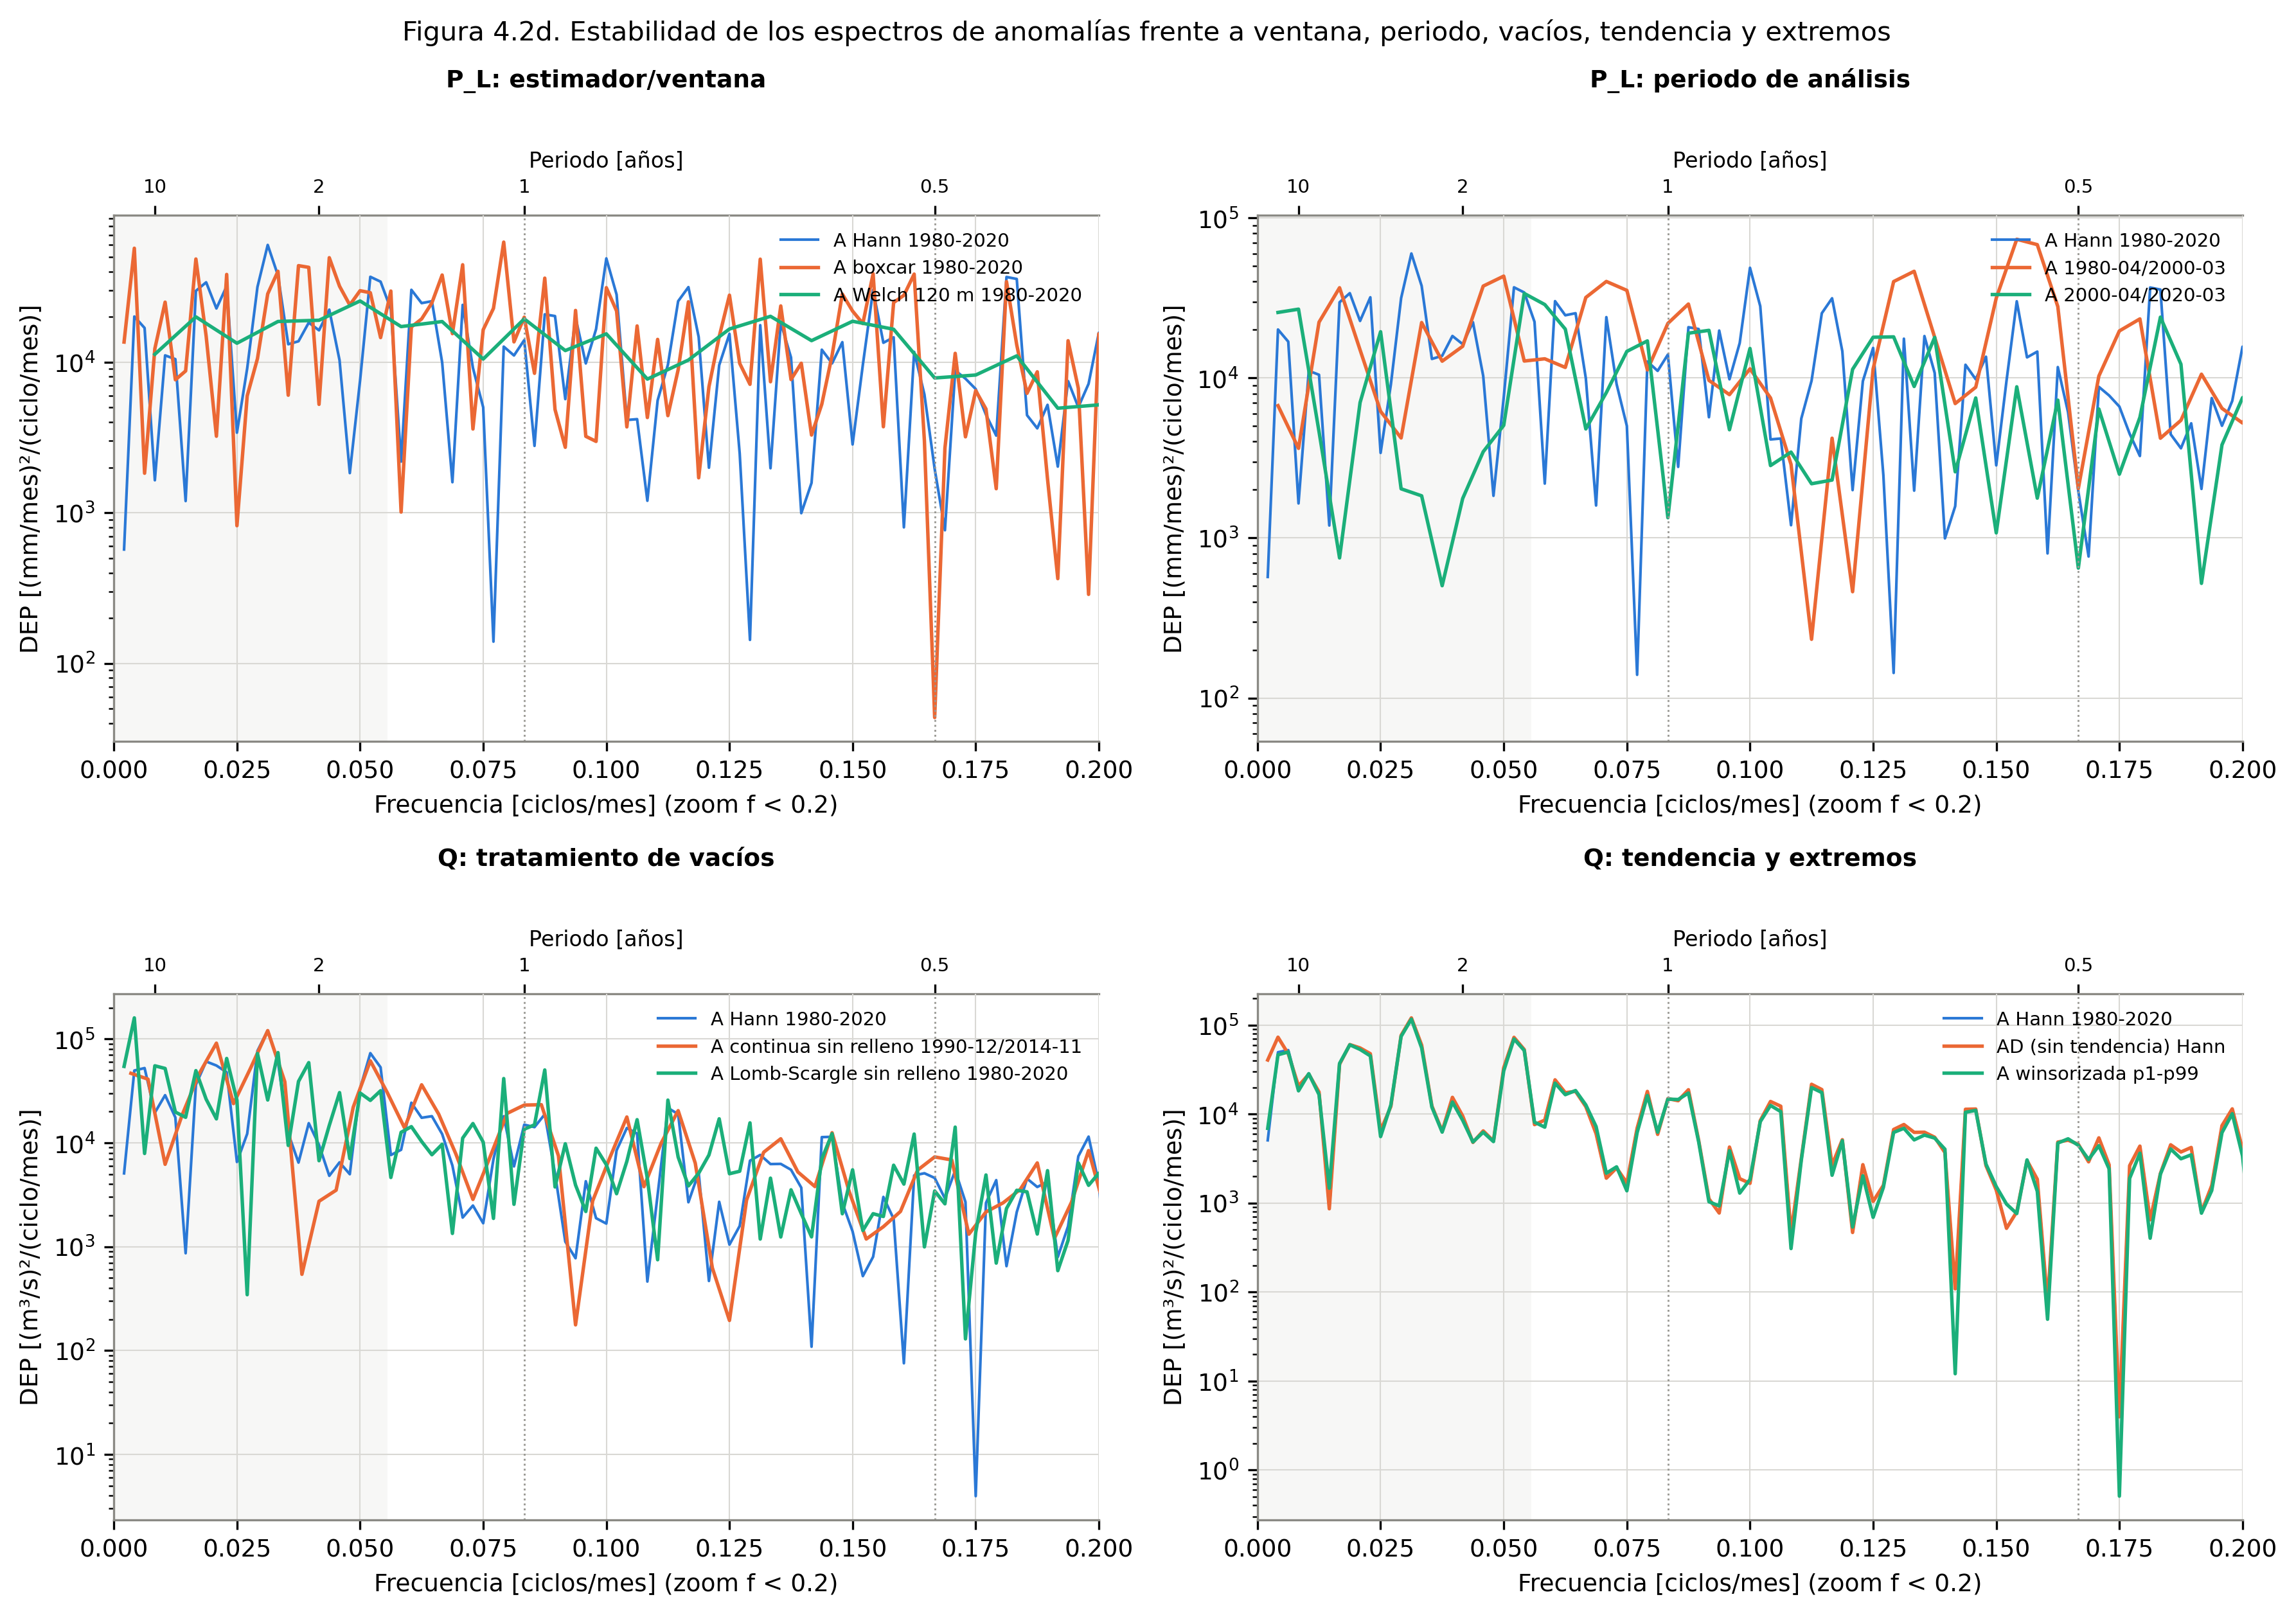
\includegraphics[width=\textwidth]{figura_4_2d_estabilidad.png}
\caption{Estabilidad de los espectros de anomalías frente al estimador, el periodo de análisis, el tratamiento
de vacíos, la tendencia y los extremos (zoom en $f<0.2$).}
\label{fig:estab}
\end{figure}

\begin{table}[H]
\centering\small
\caption{Sensibilidad del periodo interanual dominante y de la fracción interanual de varianza (anomalías).
Fuente: \texttt{figuras/tabla\_4\_2\_estabilidad\_picos.csv}.}
\label{tab:estab}
\begin{tabular}{llrr}
\toprule
Variable & Configuración & Periodo dominante [años] & Fracción interanual \\
\midrule
$P_L$ & Hann 1980--2020 & 2.7 & 0.15 \\
$P_L$ & boxcar 1980--2020 & 20.0 & 0.18 \\
$P_L$ & Welch 120 meses & 1.7 & 0.14 \\
$P_L$ & 1980-04/2000-03 & 1.7 & 0.14 \\
$P_L$ & 2000-04/2020-03 & 1.5 & 0.13 \\
$P_L$ & sin tendencia / winsorizada & 2.7 / 2.7 & 0.16 / 0.16 \\
$\overline{Q}$ & Hann 1980--2020 (relleno) & 2.7 & 0.60 \\
$\overline{Q}$ & continua sin relleno 1990--2014 & 2.7 & 0.60 \\
$\overline{Q}$ & Lomb--Scargle sin relleno & 20.0 & 0.61 \\
$\overline{Q}$ & Welch 120 meses & 3.3 & 0.53 \\
$\overline{Q}$ & 1980-04/2000-03 & 5.0 & 0.50 \\
$\overline{Q}$ & 2000-04/2020-03 & 20.0 & 0.59 \\
$\overline{Q}$ & sin tendencia / winsorizada & 2.7 / 2.7 & 0.62 / 0.61 \\
\bottomrule
\end{tabular}
\end{table}

Lo robusto es la \emph{forma} del espectro, no la ubicación de un pico interanual (Tabla~\ref{tab:estab}):
\begin{itemize}
\item \textbf{Ventana.} El periodo interanual dominante cambia de 2.7 años (Hann) a 20 años (boxcar, cuya fuga
desde la frecuencia más baja domina) o a 1.7--3.3 años (Welch). Ningún máximo interanual es estable frente al
estimador.
\item \textbf{Tendencia.} Retirarla casi no cambia el espectro del registro completo (fracción interanual de
0.60 a 0.62 en $\overline{Q}$), pero en el periodo común baja la fracción interanual del caudal de 0.56 a 0.48 y
reduce las frecuencias más bajas: en 19 años, la caída de la megasequía aparece como potencia de muy baja
frecuencia.
\item \textbf{Extremos.} Winsorizar al percentil 1--99 (lo que incluye el mayo de 1993) no altera las fracciones.
\item \textbf{Periodo.} En las dos mitades del registro el máximo interanual cambia (1.7 frente a 1.5 años en
$P_L$; 5 frente a 20 años en $\overline{Q}$), aunque la proporción de varianza interanual del caudal (0.50--0.59)
se mantiene.
\item \textbf{Vacíos.} El relleno de 14 meses no cambia el resultado: el tramo continuo y el Lomb--Scargle sin
rellenar dan la misma fracción interanual ($\approx0.60$).
\end{itemize}
Ningún pico de las anomalías supera el umbral \emph{global} del AR(1) del 95\,\%. Los que superan el umbral
puntual (32 meses en $P_L$ y $\overline{Q}$; 19 meses en $\overline{Q}$; 38 y 17.5 meses en $T$) son los esperables por
azar al examinar cientos de frecuencias (alrededor del 5\,\%), tienen pocos ciclos y no se mantienen entre
estimadores ni periodos. No se afirma ninguna periodicidad interanual significativa.

\section*{Conclusión del punto 4}

La variabilidad mensual de la cuenca se concentra en dos escalas. (1) El \textbf{ciclo anual} es la única
periodicidad significativa y estable. Domina $T$ (93\,\%) por el forzamiento radiativo; en $P_L$ (32\,\%) refleja
la estacionalidad de los sistemas frontales invernales, asociada a la migración estacional del anticiclón del
Pacífico Sur \citep{Garreaud2009}; y en $\overline{Q}$ (46\,\%) es la respuesta nival desfasada. Su armónico principal (6 meses) describe la forma no sinusoidal del ciclo y no procesos independientes. (2) Una \textbf{banda
interanual amplia}, sin picos definidos, que en el caudal reúne cerca del 60\,\% de la varianza de las
anomalías por el filtrado del almacenamiento nival, glaciar y subterráneo, y que en la precipitación es débil
(11--15\,\%). La banda de 2--7 años es compatible con la escala temporal de ENSO \citep{Trenberth1997}, que modula
la precipitación invernal de Chile central \citep{Montecinos2003} y la acumulación nival andina
\citep{Masiokas2006}. Sin embargo, un pico interanual no basta para atribuir la variabilidad a ENSO: aquí ni
siquiera hay un pico robusto, y la conexión debe evaluarse con los mapas de correlación del punto 5. Los
periodos de 20 años o más (1--2 ciclos en el registro) no se pueden distinguir de la tendencia y de la
megasequía del punto 3 y no se interpretan como oscilaciones.

\begin{thebibliography}{99}\small
% REFERENCIAS REVISADAS Y VERIFICADAS CONTRA LAS FUENTES ORIGINALES.
\bibitem{AlvarezGarreton2018} Alvarez-Garreton, C., Mendoza, P. A., Boisier, J. P., et al. (2018). The CAMELS-CL dataset: catchment attributes and meteorology for large sample studies -- Chile dataset. \emph{Hydrology and Earth System Sciences}, 22, 5817--5846. \url{https://doi.org/10.5194/hess-22-5817-2018}
\bibitem{AlvarezGarreton2021} Alvarez-Garreton, C., Boisier, J. P., Garreaud, R., Seibert, J., y Vis, M. (2021). Progressive water deficits during multiyear droughts in basins with long hydrological memory in Chile. \emph{Hydrology and Earth System Sciences}, 25, 429--446. \url{https://doi.org/10.5194/hess-25-429-2021}
\bibitem{Ayala2020} Ayala, A., Farías-Barahona, D., Huss, M., Pellicciotti, F., McPhee, J., y Farinotti, D. (2020). Glacier runoff variations since 1955 in the Maipo River basin, in the semiarid Andes of central Chile. \emph{The Cryosphere}, 14, 2005--2027. \url{https://doi.org/10.5194/tc-14-2005-2020}
\bibitem{Garreaud2009} Garreaud, R. D., Vuille, M., Compagnucci, R., y Marengo, J. (2009). Present-day South American climate. \emph{Palaeogeography, Palaeoclimatology, Palaeoecology}, 281, 180--195. \url{https://doi.org/10.1016/j.palaeo.2007.10.032}
\bibitem{Gilman1963} Gilman, D. L., Fuglister, F. J., y Mitchell, J. M. (1963). On the power spectrum of ``red noise''. \emph{Journal of the Atmospheric Sciences}, 20, 182--184. \url{https://doi.org/10.1175/1520-0469(1963)020<0182:OTPSOR>2.0.CO;2}
\bibitem{Harris1978} Harris, F. J. (1978). On the use of windows for harmonic analysis with the discrete Fourier transform. \emph{Proceedings of the IEEE}, 66, 51--83. \url{https://doi.org/10.1109/PROC.1978.10837}
\bibitem{Lomb1976} Lomb, N. R. (1976). Least-squares frequency analysis of unequally spaced data. \emph{Astrophysics and Space Science}, 39, 447--462. \url{https://doi.org/10.1007/BF00648343}
\bibitem{Masiokas2006} Masiokas, M. H., Villalba, R., Luckman, B. H., Le Quesne, C., y Aravena, J. C. (2006). Snowpack variations in the central Andes of Argentina and Chile, 1951--2005: large-scale atmospheric influences and implications for water resources in the region. \emph{Journal of Climate}, 19, 6334--6352. \url{https://doi.org/10.1175/JCLI3969.1}
\bibitem{Montecinos2003} Montecinos, A., y Aceituno, P. (2003). Seasonality of the ENSO-related rainfall variability in central Chile and associated circulation anomalies. \emph{Journal of Climate}, 16, 281--296. \url{https://doi.org/10.1175/1520-0442(2003)016<0281:SOTERR>2.0.CO;2}
\bibitem{Scargle1982} Scargle, J. D. (1982). Studies in astronomical time series analysis. II. Statistical aspects of spectral analysis of unevenly spaced data. \emph{The Astrophysical Journal}, 263, 835--853. \url{https://doi.org/10.1086/160554}
\bibitem{Torrence1998} Torrence, C., y Compo, G. P. (1998). A practical guide to wavelet analysis. \emph{Bulletin of the American Meteorological Society}, 79, 61--78. \url{https://doi.org/10.1175/1520-0477(1998)079<0061:APGTWA>2.0.CO;2}
\bibitem{Trenberth1997} Trenberth, K. E. (1997). The definition of El Niño. \emph{Bulletin of the American Meteorological Society}, 78, 2771--2777. \url{https://doi.org/10.1175/1520-0477(1997)078<2771:TDOENO>2.0.CO;2}
\bibitem{Welch1967} Welch, P. D. (1967). The use of fast Fourier transform for the estimation of power spectra: A method based on time averaging over short, modified periodograms. \emph{IEEE Transactions on Audio and Electroacoustics}, 15, 70--73. \url{https://doi.org/10.1109/TAU.1967.1161901}
\end{thebibliography}

\end{document}
